\documentclass[draftcls,onecolumn]{IEEEtran}

%% INCLUDING THE PREAMBLE
%%%%%%%%%%%%%%%%%%%%%%%%%%%%%%%%%%%%%%%%%%%%%%%%%%%%%%%%%%%%%%%%%%%%%%%%%%%
%                                                                         %
%                                 PREAMBLE                                %
%                                                                         %
%%%%%%%%%%%%%%%%%%%%%%%%%%%%%%%%%%%%%%%%%%%%%%%%%%%%%%%%%%%%%%%%%%%%%%%%%%%

%% PACKAGES
\usepackage[]{lineno}
%\linenumbers
\usepackage[usenames,dvipsnames]{xcolor}
\usepackage{microtype}
\usepackage[obeyDraft]{todonotes}
\usepackage{fancyvrb}
\VerbatimFootnotes
\usepackage{algorithmic}

%% GRAPHICS RELATED
\usepackage{graphicx}
\usepackage[outdir=./tmp/]{epstopdf}
\graphicspath{{../images/}{./}{./tmp/}}
\DeclareGraphicsExtensions{.eps, .pdf, .jpeg, .png,}

%% CPATION SETUP
\usepackage{float}
\usepackage{caption}
\usepackage{subcaption}
\captionsetup{belowskip=12pt,aboveskip=4pt}


%% BIBLIOGRAPHY
\bibliographystyle{ieeetr}

%% UNITS
\usepackage{siunitx}

%% EQUATIONS
\usepackage{amsmath}
%\numberwithin{equation}{section}

%% HYPERLINKS
\usepackage[debug]{hyperref}

%%%%%%%%%%%%%%%%%%%%%%%%%%%%%%%%%%%%%%%%%%%%%%%%%%%%%%%%%%%%%%%%%%%%%%%%%%%
%                                                                         %
%                             Listing Setup                               %
%                                                                         %
%%%%%%%%%%%%%%%%%%%%%%%%%%%%%%%%%%%%%%%%%%%%%%%%%%%%%%%%%%%%%%%%%%%%%%%%%%%
\usepackage{listings}
\lstset{ %
    language=C++,
    basicstyle=\footnotesize\ttfamily,
    numbers=left,
    numberstyle=\tiny\color{gray},
    stepnumber=2,
    numbersep=5pt,
    backgroundcolor=\color{white},
    showspaces=false,
    showstringspaces=false,
    showtabs=false,
    frame=single,
    rulecolor=\color{black},
    tabsize=2,
    breaklines=true,
    breakatwhitespace=false,
    title=\lstname,
    keywordstyle=\color{blue},
    commentstyle=\color{OliveGreen},
    stringstyle=\color{orange}
}
\DeclareCaptionFont{white}{\color{white}}
\DeclareCaptionFormat{listing}{\colorbox[cmyk]{0.43, 0.35, 0.35, 0.01}{\parbox{\dimexpr\textwidth-2\fboxsep\relax}{#1#2#3}}}
\captionsetup[lstlisting]{format=listing,labelfont=white,textfont=white,singlelinecheck=false,margin=0pt,font={bf,footnotesize}}
%\lstnewenvironment{code}[1][]%
%{ \noindent\minipage{\linewidth}
%	\lstset{#1}
%}
%{\endminipage}
%% USER COMMANDS
\usepackage{isotope}
\newcommand{\iso}{\isotope}
\newcommand{\figurewidth}{\textwidth}
\newcommand{\micron}{$\mu$m}



%%%%%%%%%%%%%%%%%%%%%%%%%%%%%%%%%%%%%%%%%%%%%%%%%%%%%%%%%%%%%%%%%%%%%%%%%%%
%                                                                         %
%                                Start of Document                        %
%                                                                         %
%%%%%%%%%%%%%%%%%%%%%%%%%%%%%%%%%%%%%%%%%%%%%%%%%%%%%%%%%%%%%%%%%%%%%%%%%%%
\begin{document}
\title{Comparison of Lithated Glass, LiF:ZnS(Ag), Boron Loaded Pastic, and PEN Films}
\author{Matthew J. Urffer}
\date{\today}
\maketitle

% Tables of Contents, Figures, Tables
\tableofcontents
\listoffigures
\listoftables
%%%%%%%%%%%%%%%%%%%%%%%%%%%%%%%%%%%%%%%%%%%%%%%%%%%%%%%%%%%%%%%%%%%%%%%%%%%
%                                                                         %
%                              Start of Content                           %
%                                                                         %
%%%%%%%%%%%%%%%%%%%%%%%%%%%%%%%%%%%%%%%%%%%%%%%%%%%%%%%%%%%%%%%%%%%%%%%%%%%
\section{Introduction}

The potential application  of a material for use in a Radiation Portal Monitor (RPM) can be indiciated by measurments of the detector's sensitivity to gammas and the neutron performance.
A detector material might be a possible replacment if the there exists a neutron response that can be differianted from gammas for given senisitivity of gammas, namely \num{1E-6}.
A simple way to discrimiante between gammas and neutrons is to have a pulse height discriminator for the gammas, above which there is only a 1 in a million chance that a gamma event will be classified as a neutron.
Under this framework, it is then possible to develop a mathmatical lower level discriminator (MLLD) to function as this pulse height discriminator, and to then formulate the senstivity requriement as the gamma intrisinic efficinecy as a function of MLLD being less than \num{1E-6}.

Six detectors (three boron loaded plastic scintillators, one LiF:ZnS(Ag) doped screen, GS20, and an annealed composite PEN film) were then evaluated for their ability to perform in a RPM. 

\begin{table}
\centering
\caption[Detector Physical Characteristics]{Physical characteristics of the detector.}
\label{tab:PhysicalProperties}
\begin{tabular}{m{3cm}| m{1cm} m{1cm} m{1cm}}
	& Absorber & Thickness &  Mass Absorber (mg) \\
EJ 254 2.5\% & \iso[10]{B} & 1/4" & 59.5 \\
EJ 254 1\% & \iso[10]{B} & 1/4" & 23.8 \\
EJ 254 5\% & \iso[10]{B} & 3/4 & 356.1 \\
EJ 425 HD2-PE & \iso[6]{Li} & \SI{0.1}{\mm} & 17.5 \\
GS20 & \iso[6]{LI} & \SI{2}{\mm} & 155 \\
Annealed Composite PEN Film & \iso[6]{Li} & $\approx$ \SI{250}{\um} & 28.1 \\
\end{tabular}
\end{table}

\subsection{Previous Work}

Work by Guerard (published slides) has published slides of the performance of GS20 and a LiF:ZnS film (\autoref{fig:GuerardLightYield}).
It should be noted for the start that Guerard's measurment is not the same as ours - the neutron source is unkown, as well is the suplier of the LiF:ZnS film (and thickness). 
In addition, the thicknes of GS20 reported by Guerard is \SI{0.5}{\mm} while the GS20 in the detection lab is \SI{2}{\mm}.
\begin{figure}
  \centering
  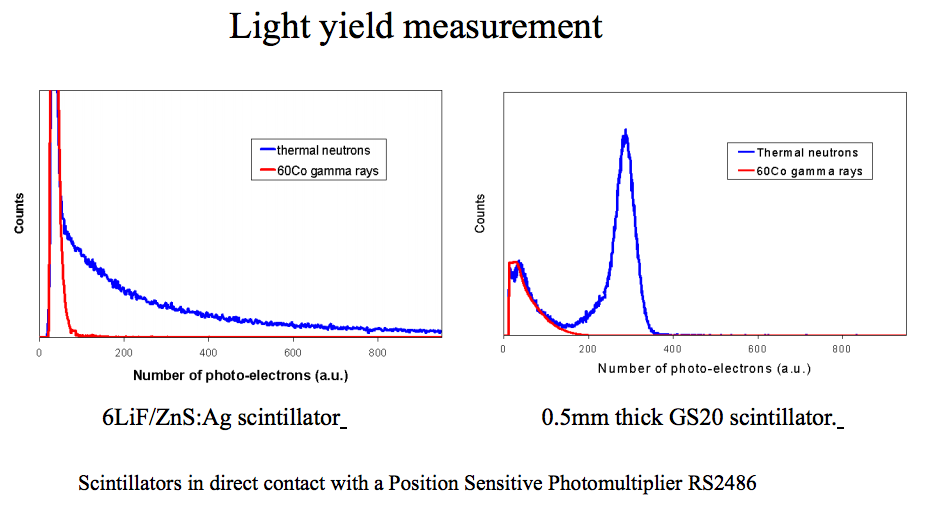
\includegraphics[width=\textwidth]{Guerard_LightYieldMeasurement}
  \caption[Measured Light Yield (Guerard)]{Light yeild as measured by Guerard. The GS20 measurement has a lower gamma performance than as measured, and the LiF:ZnS does not have the same shape as we measured}
	\label{fig:GuerardLightYield}
\end{figure}
The following figure, \autoref{fig:GuerardIntEff}, shows the neutron detection efficiency and sensitivity to \iso[60]{Co} rays.
For a senisitivity of \num{10E-6} the LiF:ZnS film is reported to have a neutron detection efficiency of 60\%, while the \SI{1}{\mm} GS20 has a reported neutron detection efficiency of 55\%.
\begin{figure}
  \centering
  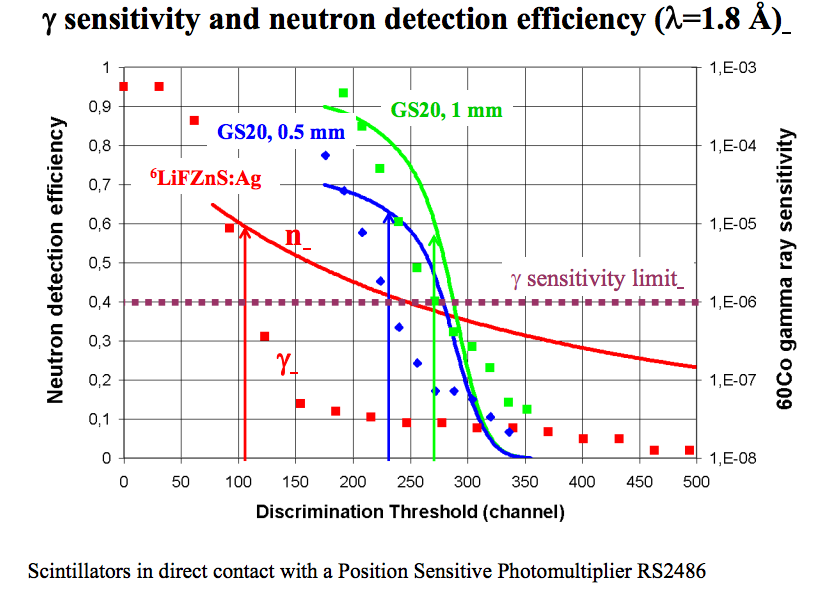
\includegraphics[width=\textwidth]{Guerard_IntEff_NCr}
  \caption[Intrisinic Efficiency (Geurard)]{Intrisinic Efficiency of LiF:ZnS and GS20 from Guerard.  The gamma intrisinic efficiency is shown in the solid squares (right axis), while the lines show the nuetron efficiency (left axis). The values reported here are much higher than the values reported in this report.}
	\label{fig:GuerardIntEff}
\end{figure}

\section{Methods}

\subsection{Mass of \iso[6]{Li} in Samples}
The mass of \iso[6]{Li} was cacluated for each of the sample in order to normalize the samples performance.


\subsection{Neutron Perfomance above Gamma Discriminator}
An accurate measure of the neturon performance above the pulse height discriminator is essential for the comparison between detector materials (\autoref{eqn:FractionAbove}).
Previous work has focused on using the fraction of neutron counts above the MLLD; however it was observed that this method (as it is normalized by the entire count rate) is very suscetible to noise in the low energy channels.
Therefore, after extensive studies using the polystyrene matrix a more stable measure was found.
\begin{align}
\label{eqn:FractionAbove}
\frac{\int_{\text{MLLD}}^\infty p(x)dx}{\int_0^\infty p(x)dx}
\end{align}
\begin{align}
\label{eqn:CountRateAbovePerMass}
\eta = \frac{\int_{\text{MLLD}}^\infty p(x)dx}{\text{Neutron Absorber Mass}}
\end{align}

\section{Results}

The average channel number of the neutron and gamma spectra of each detector was calcualted and are presented in \autoref{tab:AvgChNG}.
The average was computed for the neutrons in the thermal well to avoid the low energy channels from shifting the spectra away from any peak location.
It should be noted that for the EJ-254 theat the low channel number average is correct; the peak at this feature was indenfified as the neutron spectra.
\begin{table}
\caption[Average Channel Number of Gamma and Neutron Spectra]{Average channel number of gamma and the thermal neutron spectra .  All of the values are scaled to 1,000V, 10G.}
\begin{tabular}{c| c c c c}
	& Average Gamma Channel	& Photons per MeV & Average Neutron Channel & Photons per Neutron\\
EJ 254 2.5\%, 1/4"&	183.41	&	4034.25	&	54.06	&	644.68	\\
EJ 254 1\%, 1/4"&	216.25	&	4756.47	&	65.04	&	775.59	\\
EJ 254 5\%, 3/4"&	176.49	&	3881.87	&	39.56	&	471.80	\\
EJ 426 HD2&	1636.53	&	35995.87	&	2018.46	&	24070.77	\\
GS20 &	172.76	&	3800.00	&	524.10	&	6250.00	\\
Annealed Composite PEN&	87.63	&	1927.48	&	160.07	&	1908.87	\\
\end{tabular}
\end{table}

The count rates of the detectors are presented in \autoref{tab:CountRate} for both the thermal component as well as only in the lead well spectra.
\begin{table}
\caption[Detector Count Rate]{Count rate of the detectors in the thermal spectra as well as the lead well spectra.  The final two columns are normalize by the mass of the absorber in the material.}
\label{tab:CountRate}
\begin{tabular}{c | c c| c c}
&\multicolumn{2}{|c|}{Count Rate (cps)}&\multicolumn{2}{|c|}{Count Rate per Mass Absorber (cps per mg)} \\
& Thermal Neutrons &Lead Well & Thermal Neutrons & Lead Well\\
\hline
\hline
EJ 254 2.5\%, 1/4"&	1104	&	1869	&	18.5	&	31.4	\\
EJ 254 1\%, 1/4"&	447	&	1130	&	18.8	&	47.5	\\
EJ 254 5\%, 3/4"&	1417	&	3415	&	3.98	&	9.59	\\
EJ 42 6 HD2&	224	&	234	&	12.8	&	13.4	\\
GS20&	328	&	412	&	2.12	&	2.66	\\
Annealed Composite PEN&	176	&	195	&	6.26	&	6.93	\\

\end{tabular}
\end{table}

\autoref{tab:DiscrimPreformance} shows the discrimation performance of the tested detectors.

\begin{table}
\caption[Discrimination Performance]{Discrimination perfomrnace of the measured films}
\label{tab:DiscrimPreformance}
\begin{tabular}{c | c c}
	&	MLLD Location	&	Count Rate abover per Abosrber Mass (cps per mg)	\\
\hline
\hline
EJ 254, 2.5\% B, 1/4"	&	1280	&	0.20	\\
EJ 254, 1\% B, 1/4"	&	1300	&	0.05	\\
EJ 254, 5\% B, 3/4"	&	1290		&	0.03	\\
EJ 426 HD2, \SI{0.1}{\mm}&	3308		&	1.97	\\
GS20, \SI{2}{\mm}	&	557		&	0.56	\\
Annealed Composite PEN, $\approx$ \SI{250}{\um}	&	209	&	1.96	\\
\end{tabular}
\end{table}


\subsection{Agreement to Previous Results}
It is observed from \autoref{fig:GuerardIntEff} that the neutron spectra has the same endpoint while the gamma sensitivity increases with thickness.
Assuming a linear increase in the gamma sensitity with thickness, a \SI{2}{\mm} would then be expected 

\subsection{Stability of Determing Gamma LLD}
\begin{figure}


\end{figure}

\section{Conclusions}

\section{Appendix}
The EJ-254, EJ-426, GS20, and annealed composite PEN spectra data contained in this report may be found at \verb+Dropbox/SpectraFiles/(0)_2013_Data/SampleComparison_28Apr2013+.
These files were measured from April 28, 2013 to May 2, 2013.

\end{document}
